\subsection{Introduction}
The Graph Theory is one of the main tools used to infer how the brain works. A graph is a mathematical object defined
by combining \textbf{nodes} \(V\) (or vertices) and \textbf{edges} \(E\) (or arcs) connecting the nodes.
\begin{figure}[H]
    \centering
    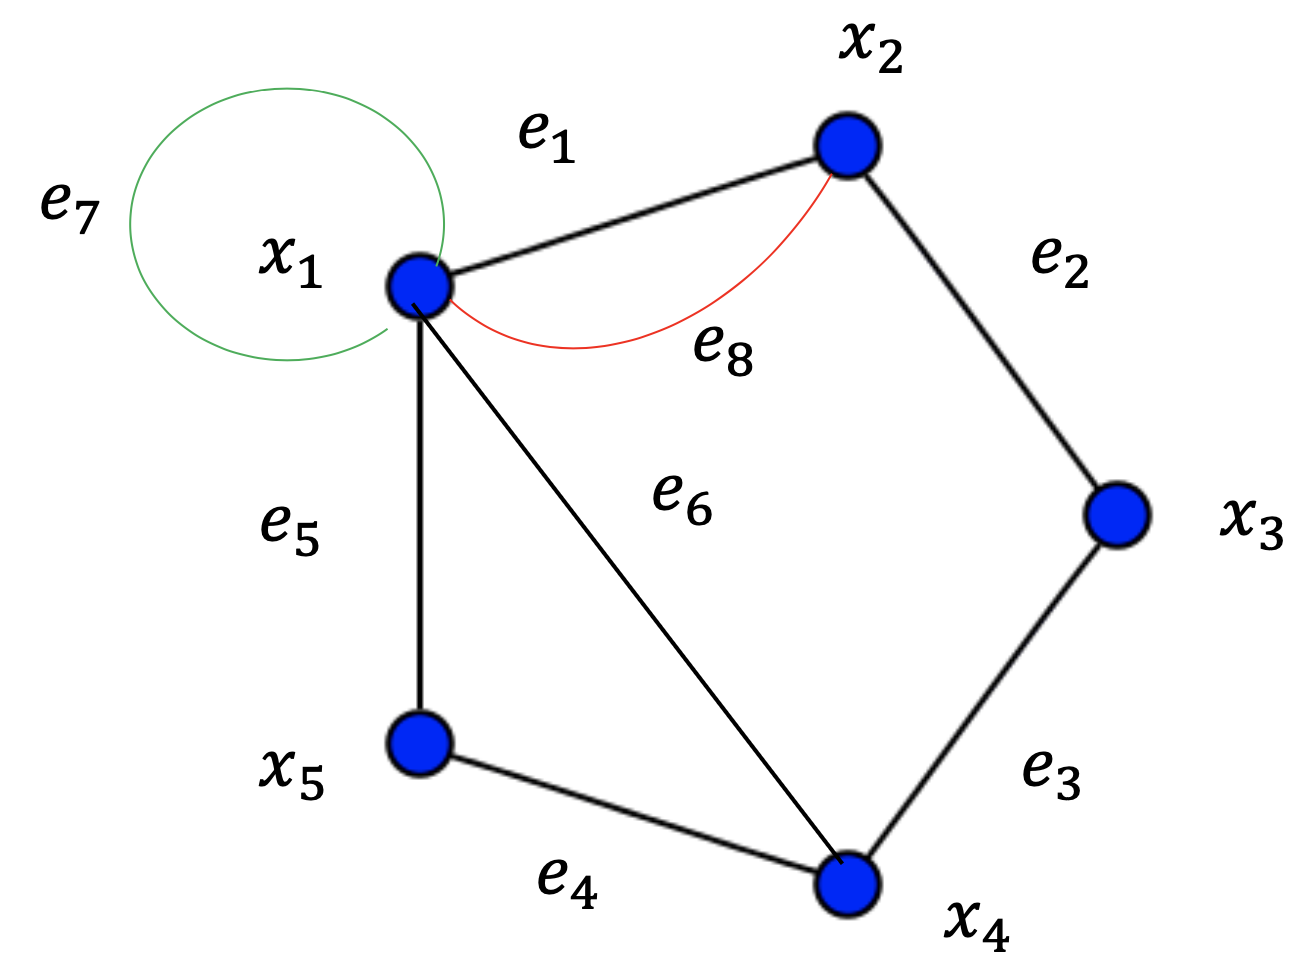
\includegraphics[scale=0.25]{15_1}
\end{figure}
\begin{equation*}
    G=(V,E)
\end{equation*}
\begin{equation*}
    V=\{x_1, x_2, ..., x_n\}
\end{equation*}
\begin{equation*}
    E=\{\{x_1, x_2\}, \{x_2,x_3\},..., \{x_{n-1},x_n\}\}
\end{equation*}
\subsubsection{Definitions}
\begin{enumerate}
    \item A node \(x_i\) is adjacent to \(x_j\) if they are connected by an edge.
    \item An edge \(\{x_i, x_j\}\) is incident with a node - i.e., \(x_i\) or \(x_j\) - if that vertex is an endpoint
          for the edge.
    \item The number of edges incident to a node is called \textbf{degree} of the node.
    \item A graph \(G=(V,E)\) with neither loops nor multiple edges is said to be \textbf{simple} (all of the graphs in
          the following will be simple).
    \item An edge \(\{x_i,x_i\}\) incident to the same node \(x_i\) is named \textbf{loop}.
    \item Two or more edges \(\{x_i,x_j\}\) incident to the same pair of nodes are called \textbf{multiple edges}
          (a.k.a. multi-edges).
\end{enumerate}
\subsubsection{Common Graphs}
There are many different topographies depending on the number of nodes and on how they are connected.
\begin{figure}[H]
    \setcounter{subfigure}{0}
    \centering
    \subfigure[]{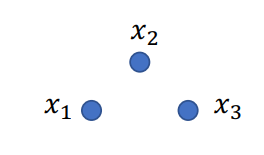
\includegraphics[width=0.2\textwidth]{15_2}}
    \subfigure[]{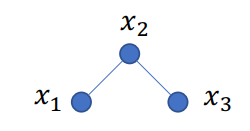
\includegraphics[width=0.2\textwidth]{15_3}}
    \subfigure[]{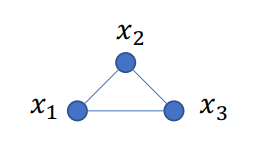
\includegraphics[width=0.2\textwidth]{15_4}}
    \subfigure[]{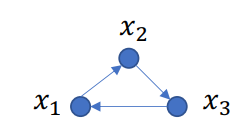
\includegraphics[width=0.2\textwidth]{15_5}}
\end{figure}
\begin{itemize}
    \item[\textbf{(a)}] \textbf{Null or empty graph}: formed only by nodes and no edges.
        \begin{equation*}
            E=\emptyset
        \end{equation*}
    \item[\textbf{(b)}] \textbf{Binary Graph}: each edge has two possible values, 0 or 1. 0 means that it is not present and 1 that it is present.
        \begin{equation*}
            E=\{\{x_1, x_2\}, \{x_2,x_3\},..., \{x_{n-1},x_n\}\},\hspace{0.5cm}e\in[0,1];
        \end{equation*}
    \item[\textbf{(c)}] \textbf{Weighted Graph}: every node is connected to the others (graph fully connected) with a certain strength, denoted
        by a certain edge weight.
        \begin{equation*}
            E=\{\{x_1, x_2\}, \{x_2,x_3\},..., \{x_{n-1},x_n\}\},\hspace{0.5cm}e\in[0,\infty];
        \end{equation*}
    \item[\textbf{(d)}] \textbf{Directed Graph}: every node is connected to the others (graph fully connected), and information on the direction of
        the connections - i.e., edges - is present.
        \begin{equation*}
            E=\{\{x_1, x_2\}, \{x_2,x_3\},..., \{x_{n-1},x_n\}\},\hspace{0.5cm}e\in[-\infty,\infty];
        \end{equation*}
\end{itemize}
PLV and Coherence are examples of weighted graphs, because they are symmetric and do not contain information about directionality.

\subsection{Connectivity Matrices and Brain Graphs}
\paragraph{How can brain observations between different scales be compared?} Graphs are a tool to collect an
abstract representation, that allows to compare network properties independently of the scale at which they
have been observed (at the single neuron level or at the network level, for instance) and to compare
signals obtained using different modalities - i.e., fMRI, electrophysiology, and metabolic imaging -.\\
Henceforth, a crucial trask is constructing a brain graph. The simplest definition would be to have nodes
coincident with the neuronal ensembles that are being recorded. However, the situation becomes more
complicated when multiple recordings are combined. Nodes can in fact be micro-, meso- or macroscopic and
it is always possible to make comparisons across different scales, but in the first place it is necessary
to understand how nodes are defined in each scale and how this definition is related to the ones in the other scales.\\
The simplest way to represent nodes is by using \textbf{adjacency matrices}: they are matrices that define the pairwise
correlation between every node in the network.
\begin{figure}[H]
    \centering
    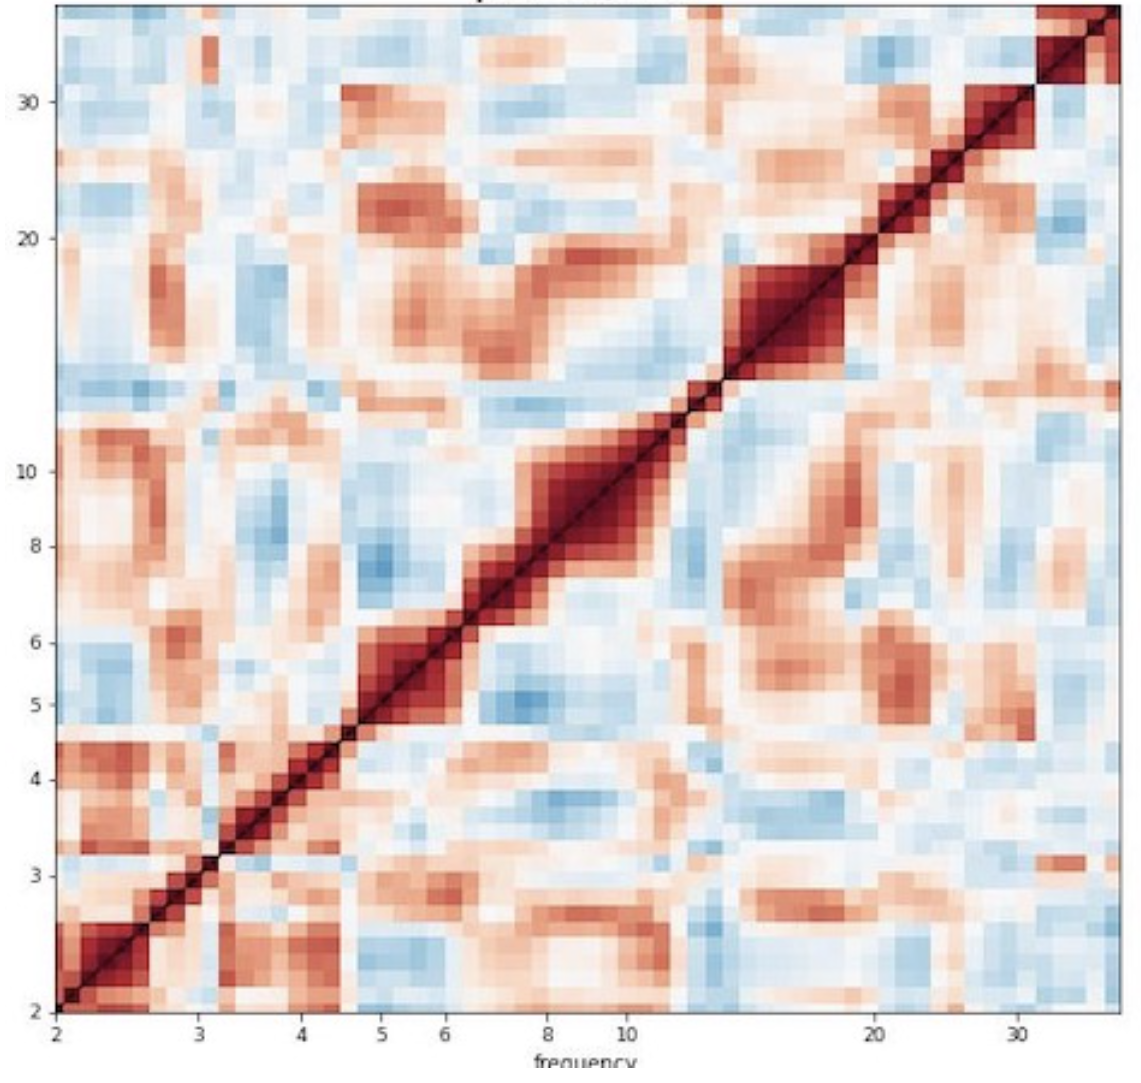
\includegraphics[scale=0.25]{15_6}
\end{figure}
A typical adjacency matrix of a brain network shows the highest values of correlation near the main diagonal,
where the close electrodes show the largest correlation, then there are clusters of connections that show
the correlation between far apart brain areas.\\
If the matrix does not show this hierarchical modular structure it is likely that there is an error in the algorithm
or that the subject suffers from some pathological condition.\\
Starting from this matrix, a lot of information can be extracted.
\subsubsection{Measures of Node Connectivity}
The node connectivity quantifies how much a single node is connected to all the others.\\
The simplest way to evaluate it is to compute the \textbf{node degree}, which is the number of incident edges:
\begin{equation*}
    k_i=\sum_{i\neq{j}}{a_{i,j}}
\end{equation*}
The \textbf{node strength} is similar to the node degree and is given by the sum of the weights of the edges
connected to a specific node, thus it makes not really sense to compute it for binary graphs:
\begin{equation*}
    s_i=\sum_{i\neq j}w_{i,j}
\end{equation*}
The \textbf{network density} is the number of non-null edges that are present w.r.t. the maximum number of possible edges.
It only makes sense in binary graphs, because in weighted graphs all the nodes are connected to one another and
there is just a difference in the connection weight.
\begin{align*}
    \text{Network potential connections} & \hspace{1.5cm}PC=\frac{N\cdot{(N-1)}}{2}     \\
    \text{Network actual connections}    & \hspace{1.5cm}AC                             \\
    \text{Network density}               & \hspace{1.5cm}ND              =\frac{AC}{PC}
\end{align*}
The network density can alternatively be defined by exploiting the node degree property:
\begin{align*}
    \text{Network maximum degree} & \hspace{1.5cm}MD=N\cdot{(N-1)}     \\
    \text{Network actual degree}  & \hspace{1.5cm}AD=\sum_{i=1}^{N}k_i \\
    \text{Network density}        & \hspace{1.5cm}ND=\frac{AD}{MD}
\end{align*}
The \textbf{clustering coefficient} of a single node \(x_i\) is the number of nodes \(x_j\) that are both adjacent to
\(x_i\) and adjacent to each other. It tells how much one node is central for the considered network, thus it provides
a hint about how modular the network is.
\subsubsection{Degree Distribution}
The degree distribution term indicates the probability of having one node connected to other nodes. It applies very well
to large networks - i.e., \(>1000\) nodes -. By looking at it, information about the actual topography of a network
can be inferred. In \textbf{single-scale graphs} (Erdos-Renyi) the degree distribution follows a binomial distribution
that for large values of \(n\) tends to a Gaussian.
\begin{align*}
    Pr(deg(x)=k) & = \begin{pmatrix}
                         N+1 \\
                         k
                     \end{pmatrix}
    p^k(1-p)^{N-1-k}
\end{align*}
\textbf{Scale-free graphs} (brain and all biology-inspired systems) follow a power-law distribution, suggesting the
presence of large hubs, being nodes very connected.
\begin{equation*}
    Pr(deg(x)=k)=k^{-\alpha}
\end{equation*}
\textbf{Broad-scale graphs} (social networks) follow a truncated power-law - i.e., a combination of exponential and
binomial distributions -.
\begin{equation*}
    Pr(deg(x)=k)=k^{-\alpha}e^{-k/k_c}
\end{equation*}
\subsubsection{Centrality and Hubs}
Looking at scale-free distributions, it can be deduced that some nodes have a very important role in ensuring the
stability of the network, as they play a central role: such nodes are named hubs\\
Hubs have a very high clustering coefficient, as they are connected to large amounts of nodes:
the majority of the nodes can communicate with each other only by passing through hubs.\\
Hence, nodes exhibiting a high degree of centrality are distinguished by three properties:
\begin{enumerate}
    \item Maximum possible degree.
    \item They are included in the shortest possible topological path between two other nodes.
    \item They are located at the shortest distance from all the other nodes.
\end{enumerate}
\begin{figure}[H]
    \centering
    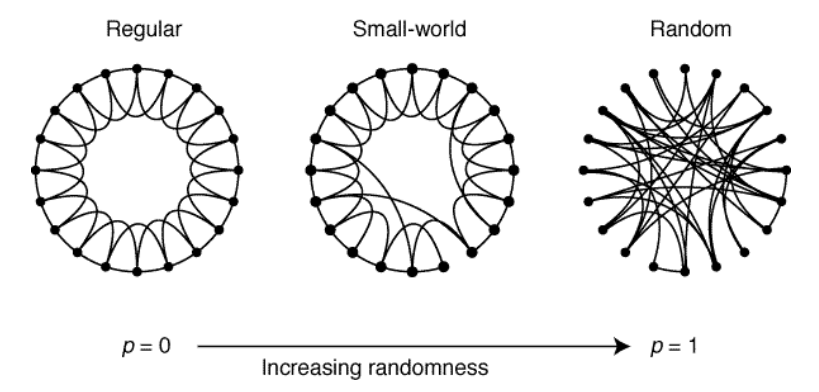
\includegraphics[scale=0.8]{15_7}
\end{figure}
Let's consider the following example: an epileptic network could be treated surgically, by removing or disconnecting the
nodes that are central for the propagation or the creation of epilepsy.\\
Based on these observation, the three cardinal aspects of \textbf{centrality} are: degree, betweenness and closeness.
These are used to easily identify these regions.
\begin{itemize}
    \item \textbf{Degree Centrality} is equivalent to node degree.
    \item \textbf{Eigenvector Centrality} takes into account the degree of a node and those of its neighbours are computed
          by eigen-decomposing it:
          \begin{equation*}
              C_e(i)=\frac{1}{\lambda_1}\sum_{j=1}^NA_{ij}x_j
          \end{equation*}
    \item \textbf{Closeness Centrality} is the inverse of the average shortest path length, that is the lower number
          of edges that one has to pass to go from one side of the network to the other.
          \begin{equation*}
              C_c(i)=\frac{N-1}{\sum_{j\neq i}l_{ij}}
          \end{equation*}
    \item \textbf{Betweenness Centrality} measures the proportion of shortest paths between all the nodes pairs in a
          network passing through a given node. Thus, it measures how much a single node is central in a large population.
          \begin{equation*}
              C_b(i)=\frac{1}{(N-1)(N-2)}\sum_{h\neq i,h\neq j, j\neq i} \frac{\rho_{hj}(i)}{\rho_{hj}}
          \end{equation*}
\end{itemize}
As already said, biological networks are characterized by skewed degree distributions suggesting the existence of highly
connected nodes, called hubs.
\paragraph{How can hubs be detected in brain networks?} In 2007, Sporns suggested that they are characterized by:
\begin{enumerate}
    \item \textbf{High degree}, implying they are connected to many nodes;
    \item \textbf{High closeness centrality}, thus they support communication between nodes;
    \item \textbf{High betweenness and low clustering}, then supporting the integration of unconnected nodes.
\end{enumerate}
In 2010, Van den Heuvel applied a similar approach to classify brain regions based on their centrality with respect to
the human connectome for each node. The node is categorized as a hub if:
\begin{enumerate}
    \item It is ranked in the top \(20\%\) among those with \textbf{highest degree}.
    \item It is ranked in the top \(20\%\) among those with \textbf{highest betweenness}.
    \item It is in the bottom \(20\%\) with the \textbf{lowest clustering coefficient}.
    \item It is in the bottom \(20\%\) among those with the \textbf{lowest average path length}.
\end{enumerate}

\subsection{Graphs Interpretation and Labelling}
Interpreting graphs is usually very difficult, a lot of nodes are often connected together. Therefore, to extrapolate
information from them it is necessary to perform some meaningful labelling.\\
To do so, labels are assigned according to the properties of the nodes. In brain networks, modules are looked for, as they
are clusters of nodes sharing similar properties.
\subsubsection{Modularity}
\begin{figure}[H]
    \centering
    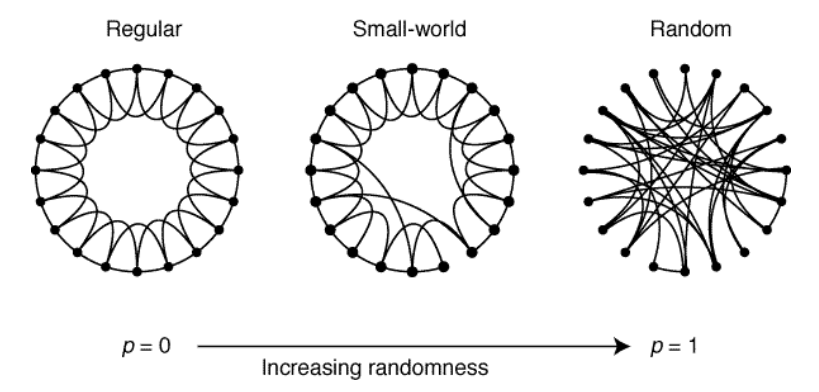
\includegraphics[scale=0.7]{15_8}
\end{figure}
Generally, modular networks such as the human brain have small-world properties, in particular high clustering coefficients
and low characteristic path lengths.\\
This means there is a group of highly connected nodes and then a hub, such that the information can reach all the other
possible portions of the network by passing through this hub. This topography is optimal for energy conservation, speed
of communication, and general economy of the brain.\\
The basic idea to perform modularity is to reduce a large set of observations across different measures into a smaller
subset of informative clusters. However, the number of natural clusters is not known \textit{a priori}. Hence, techniques
like multidimensional scaling or PCA are often used. In general, data clustering methods can be divided in two classes:
\textbf{agglomerative}, which starts from the part in which nodes share the same properties, and \textbf{divisive},
starting from a larger view of the whole network.
\subsubsection{Agglomerative Modularity}
In agglomerative modularity, the nodes sharing the same properties are combined starting from a small portion
of the network.\\
\textbf{Hierarchical clustering} groups nodes in clusters to promote high within-cluster similarity and low
between-clusters similarity. It is an iterative algorithm in which, at the beginning, all nodes belong to their own cluster
(singletons), then nodes with the highest similarity and groups of nodes with the highest similarity are joined in an iterative
fashion.\\
Two possible implementations of hierarchical clustering algorithms are the Average-linkage clustering and Single-linkage
(or Complete-linkage) clustering.
\subsubsection{Divisive Modularity}
In divisive modularity the network is cut into small portions.
It is based on betweenness centrality: the betweenness is calculated for each edge in the graph, then the edges
that have the highest score are removed by cutting the network at that point. Then, the process is repeated until there are
no more edges in the graph.\\
Depending on where the graph is cut, a highly variable number of clusters can be obtained. When deciding where to cut, some
factors are to be considered:
\begin{itemize}
    \item Optimize neighbouring proximity of nodes.
    \item Use algorithms that provide the confidence intervals (obtained through statistical analyses) on where the
          network can be cut.
\end{itemize}
To sum up, the usage of agglomerative or divisive modularity is a good way of proceeding, since it does not require
an \textit{a priori} selection of the exact number of clusters that will be extracted from data. However, there is no
easy way to determine the quality of the obtained clusters. To do so, often permutations are used to estimate the
confidence intervals.
\paragraph{How can modularity be quantified?} A high-quality partition should have:
\begin{itemize}
    \item Highly-cohesive modules or strongly connected nodes within the same module.
    \item A larger intra-modules connectivity than the one expected by chance (when edges are placed at random).\\
          To evaluate it, the \textbf{modularity index} can be defined as:
          \begin{equation*}
              Q=\frac{1}{2}A_{ij}\delta(m_i,m_j)
          \end{equation*}
          This value is dependent on the point where the system is cut, thus it should be calculated for
          different thresholds. Then, the value that maximizes the modularity is chosen.
          The Louvain method is an algorithm that can be used to maximize the modularity index.
\end{itemize}

\subsection{Null Models}
As already introduced for the PLV or the PSTH, the evaluation of a single parameter is meaningful only in the
presence of a null hypothesis. This means that measuring a clustering coefficient of the brain network of 0.4
and an average path length of 4 is not particularly informative in the absence of comparative information - i.e.,
the null hypothesis -.
As a matter of fact, in brain networks the edges are not placed randomly, but they follow specific anatomical
directions. Hence, a good way to proceed would be to compare the results of a given brain network with another
random brain network.\\
The simplest form of random network is the Erdos-Renyi model, though other models exist as well.
\subsubsection{The Erdos-Renyi Model}
Even if this model is very simple, unluckily it is not really comparable to real brain networks because
it is not a small-world network, since it exhibits long-range connections which are very expensive in terms
of energy consumption and topographical characteristics very different from the ones that exist in the brain.\\
To build this model:
\begin{enumerate}
    \item Distribute \(N\) nodes in a random topology.
    \item Pick a random (uniform) number between 0 and 1.
    \item If this is greater than the probability \(p\) (a model parameter), draw an edge between
          \(x_i\) and \(x_j\).
    \item Repeat for all the \(N\) nodes.
\end{enumerate}
Notice that \(m\) edges are obtained and \(2^m\) different models can be generated by changing the
vertices connected to the edges.
\subsubsection{The Watts-Strongatz Model}
Here the degree distribution is Poisson-like, which is unrealistic if compared to real-world networks.
\begin{enumerate}
    \item Begin with \(N\) nodes in a 2D space positioned on a ring and a desired mean node
          degree \(\langle{k}\rangle\). Choose \(\langle{k}\rangle\) as an even number.
    \item Add \(N\langle{k}\rangle/2\) edges to a given node, \(\langle{k}\rangle/2\) on each side,
          between its \(\langle{k}\rangle\) nearest neighbours.
    \item Randomly rewire each connection with a probability \(0<p<1\), avoiding loops and multi-edges.
    \item Notice that \(p=0\) yields a Erdos-Renyi model for \(N\) nodes.
\end{enumerate}
\subsubsection{The Barabasi-Albert Model}
This approach yields a graph with a degree distribution that follows a power-law and has a connection
density of \(2v/(N-1)\).
\begin{enumerate}
    \item Nodes are not fixed, rather added at each iteration.
    \item Begin with a few interconnected nodes.
    \item At each iteration, add a new node with preferential attachment, meaning that a new node added
          to the graph will be preferentially connected to highly connected nodes already present in the
          graph.
\end{enumerate}
\subsubsection{The Maslov-Sneppen Rewiring}
This model has been defined as a surrogate for comparisons with neuronal networks. It was specifically
built for binary graphs:
\begin{enumerate}
    \item It takes the graph and iteratively rewires each edge.
    \item At each iteration it randomly selects two edges \(\{x_1,x_2\}\) and \(\{x_3,x_4\}\)
    \item Then it changes these edges to form \(\{x_1,x_4\}\) and \(\{x_2,x_3\}\).
    \item If one of the edges already exists, it is dropped.
    \item The algorithm iterates for a fixed number of repetitions. This number is usually exceeding by
          100 times the number of existing edges.
\end{enumerate}
This method yields a graph with the same size, average node degree, and degree distribution as the original one.\\
Its advantage is that it is simple to implement but quite expensive for very large networks.

\subsection{The Critical Brain Hypothesis}
Statistical mechanics is a branch of theoretical physics studying the average behaviour of mechanical
systems where the state of the system is uncertain. Thanks to it, complex systems with many (up to \(10^{23}\))
degrees of freedom can be described.\\
The brain is thought to operate in a \textbf{sub-critical regime near the critical point} in
physiological conditions. This critical point is seen as the point of transition between two states.\\
Self-Organized Criticality (SOC) is a property of dynamical systems which have a critical point as an
attractor. In this field, systems are predicted to exhibit scale-invariant characteristics or power-laws.\\
Complex systems can generate extremely complex dynamics. The global behaviour of the network originates
from local interactions, in absence of a single generator. The dynamic behaviour of the brain network
can be observed for every brain time serie. One simple way to do it is through the large-scale neuronal
avalanches.
\subsubsection{Large-Scale Neuronal Avalanches}
In dynamical systems the activity propagates from one region to another with different travelling waves.
Large-scale neuronal avalanches are the simplest way to characterize travelling waves. Neuronal
avalanches are described in terms of their spatial extent and life-time. Both these properties follow a
power-law in physiological conditions, whenever the brain is operating near the critical point.
Starting from the avalanches, the so-called propagation matrix can be extracted.
\begin{figure}[H]
    \centering
    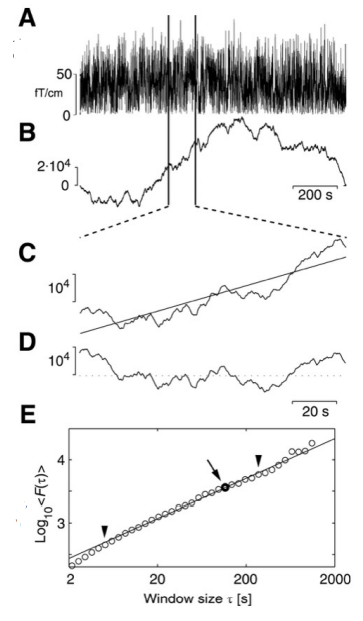
\includegraphics[scale=0.42]{15_9}
\end{figure}
One way to measure neuronal avalanches in large-scale activity is to look at the activity at different
sides of the brain: after filtering in a specific band and taking the module of the complex wavelet,
the amplitude dynamics can be extracted. Then, an amplitude threshold is defined and only the nodes
whose amplitude is above the threshold are considered as active.\\
This is performed for a single value to have a single element in the matrix or for many temporal windows
and amplitude thresholds in order to quantify the network large activation. The values depicted in yellow
in the previous figure follow exactly a power-law and define the critical regime, that is the portion of
the network where the communication is optimal.
\subsubsection{Long-Range Temporal Correlations}
The brain spontaneously generates neuronal oscillations with great variability in terms of frequency,
duration, and amplitude. Little is known w.r.t. their long-term temporal structure. Since the brain has
memory, it should exhibit some sort of long-term temporal correlation.\\
To analyze this quantity, the simplest analysis to perform is the \textbf{Detrend Fluctuation Analysis} (DFA).\\
This algorithm relies on the assumption that whether a critical system works at the optimal state point,
then it has the maximum possible - i.e., thw best - DFA. By increasing or decreasing this value after any particular
condition means that the critical point is moving away, towards more excitatory or inhibitory states.
\begin{figure}[H]
    \centering
    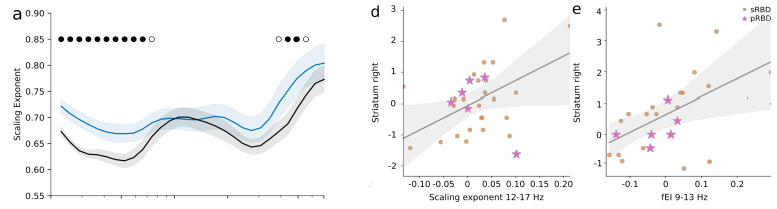
\includegraphics[scale=0.82]{15_10}
\end{figure}
To realize this algorithm, after measuring the activity in one point, the amplitude modulation is
taken, then a cumulative distribution of this amplitude is generated. Later, by considering a smaller
time window, the linear trend within it is quantified and removed. This is repeated for different time
windows, obtaining different linear fittings. The DFA is finally defined as the linear or power-law
fitting of the curve built from the amplitude dynamics observed at different time windows. This technique
is long-range because very large time windows (\(2000\,s\)) are also considered.\\
When the DFA changes, different interpretations can be hypothesized.
\begin{figure}[H]
    \centering
    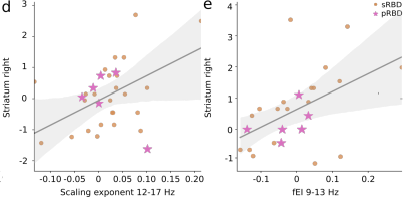
\includegraphics[scale=0.6]{15_11}
\end{figure}
\paragraph{Example} In this study, the DFA computed across multiple frequencies (\(2-70\,Hz\)) of
patients with a sleeping disorder and a healthy control group is observed. These subjects have
significantly different values in the low frequency range. Such a change is correlated to a clinical
index in the patients pathology that is the dopaminergic loss: increases of DFA for the healthy control
group is directly correlated with the dopaminergic loss.
